\documentclass[border=2pt]{standalone}
\usepackage{tikz}
\usetikzlibrary{arrows.meta,positioning}
\begin{document}
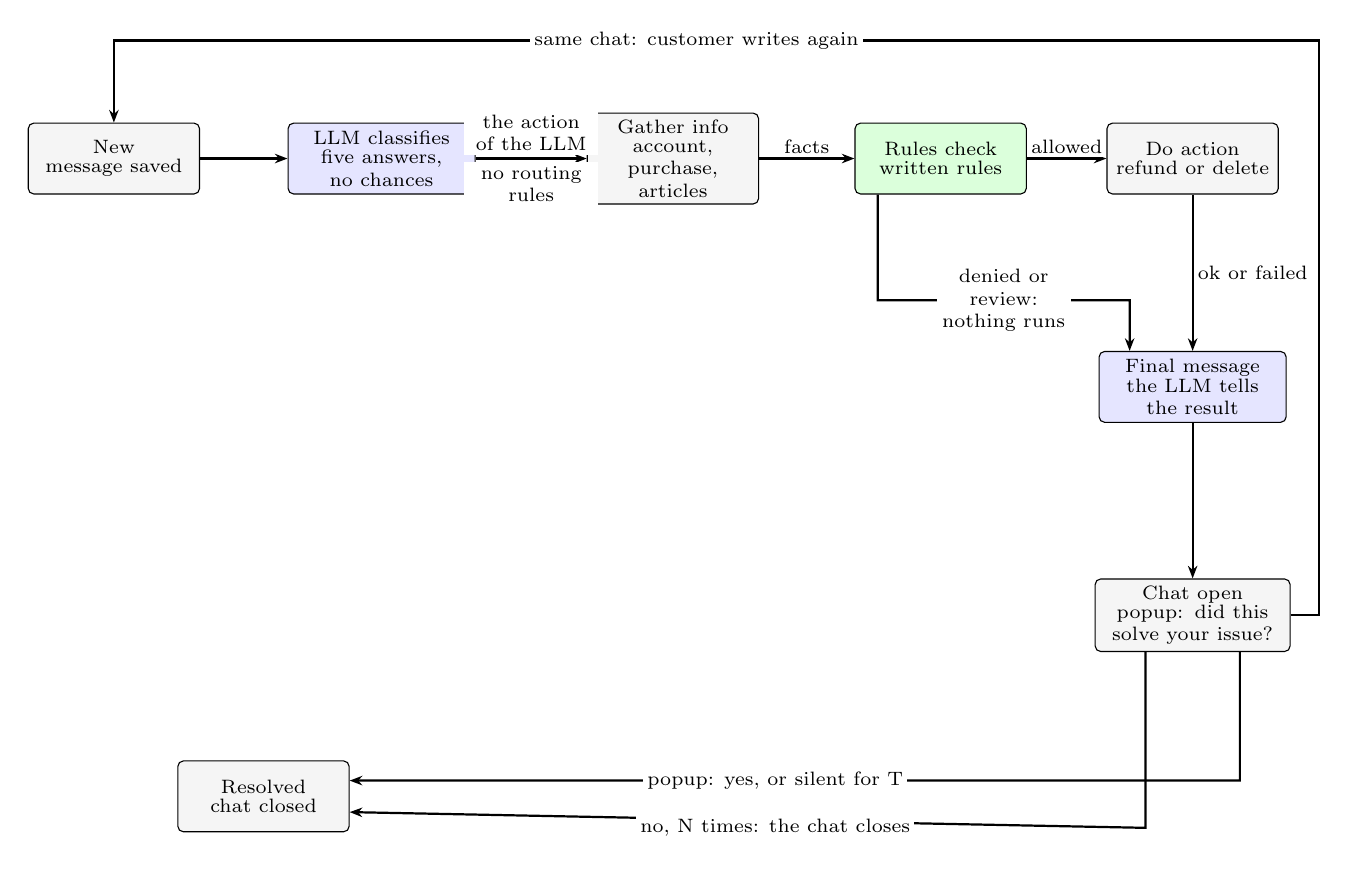
\begin{tikzpicture}[
  every node/.style={font=\scriptsize},
  st/.style={draw, rounded corners=2pt, minimum height=9mm, text width=20mm, align=center, inner sep=2.5pt},
  fx/.style={st, fill=gray!8},
  md/.style={st, fill=blue!10},
  rl/.style={st, fill=green!14},
  ar/.style={-{Stealth[length=1.6mm]}, thick},
  lb/.style={font=\scriptsize, inner sep=1.5pt, fill=white, text width=16mm, align=center},
  lw/.style={font=\scriptsize, inner sep=1.5pt, fill=white}]
  \coordinate (yt) at (0,1.5);
  \node[fx] (new) at (0,0) {New\\[-1pt]{\scriptsize message saved}};
  \node[md, text width=22mm] (llm) at (3.4,0) {LLM classifies\\[-1pt]{\scriptsize five answers, no chances}};
  \node[fx] (gat) at (7.1,0) {Gather info\\[-1pt]{\scriptsize account, purchase, articles}};
  \node[rl] (rul) at (10.5,0) {Rules check\\[-1pt]{\scriptsize written rules}};
  \node[fx] (act) at (13.7,0) {Do action\\[-1pt]{\scriptsize refund or delete}};
  \node[md, text width=22mm] (fin) at (13.7,-2.9) {Final message\\[-1pt]{\scriptsize the LLM tells the result}};
  \node[fx, text width=23mm] (cha) at (13.7,-5.8) {Chat open\\[-1pt]{\scriptsize popup: did this solve your issue?}};
  \node[fx] (res) at (1.9,-8.1) {Resolved\\[-1pt]{\scriptsize chat closed}};

  \draw[ar] (new) -- (llm);
  \draw[ar] (llm) -- node[lb, above=1pt]{the action of the LLM} node[lb, below=1pt]{no routing rules} (gat);
  \draw[ar] (gat) -- node[lw, above]{facts} (rul);
  \draw[ar] (rul) -- node[lw, above]{allowed} (act);
  \draw[ar] (act) -- node[lw, right]{ok or failed} (fin);
  \draw[ar] ([xshift=-8mm]rul.south) -- (9.7,-1.8) -- (12.9,-1.8) -- ([xshift=-8mm]fin.north);
  \node[lb] at (11.3,-1.8) {denied or review: nothing runs};
  \draw[ar] (fin) -- (cha);
  \draw[ar] ([xshift=6mm]cha.south) -- (14.3,-7.9) -- ([yshift=2mm]res.east);
  \node[lw] at (8.4,-7.9) {popup: yes, or silent for T};
  \draw[ar] ([xshift=-6mm]cha.south) -- (13.1,-8.5) -- ([yshift=-2mm]res.east);
  \node[lw] at (8.4,-8.5) {no, N times: the chat closes};
  \draw[ar] (cha.east) -- (15.3,-5.8) -- (15.3,1.5) -- (new.north |- 0,1.5) -- (new.north);
  \node[lw] at (7.4,1.5) {same chat: customer writes again};
\end{tikzpicture}
\end{document}
